\tikzset{every picture/.style={line width=0.75pt}} %set default line width to 0.75pt        

\begin{tikzpicture}[x=0.75pt,y=0.75pt,yscale=-1,xscale=1]
%uncomment if require: \path (0,300); %set diagram left start at 0, and has height of 300

%Straight Lines [id:da40044393626129515] 
\draw    (189,141) -- (253,141) ;
\draw [shift={(256,141)}, rotate = 180] [fill={rgb, 255:red, 0; green, 0; blue, 0 }  ][line width=0.08]  [draw opacity=0] (8.93,-4.29) -- (0,0) -- (8.93,4.29) -- cycle    ;
\draw [shift={(186,141)}, rotate = 0] [fill={rgb, 255:red, 0; green, 0; blue, 0 }  ][line width=0.08]  [draw opacity=0] (8.93,-4.29) -- (0,0) -- (8.93,4.29) -- cycle    ;
%Image [id:dp06489700122042041] 
\draw (319.5,139.7) node  {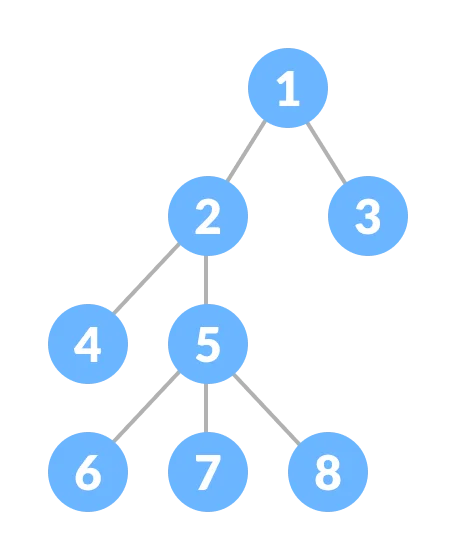
\includegraphics[width=95.25pt,height=114.15pt]{images/arbol.png}};
%Image [id:dp03981772270142003] 
\draw (550.2,142.2) node  {
\includegraphics[width=136.8pt,height=75.6pt]{images/data.jpg}};
%Image [id:dp7011475910977688] 
\draw (100.3,136.3) node  {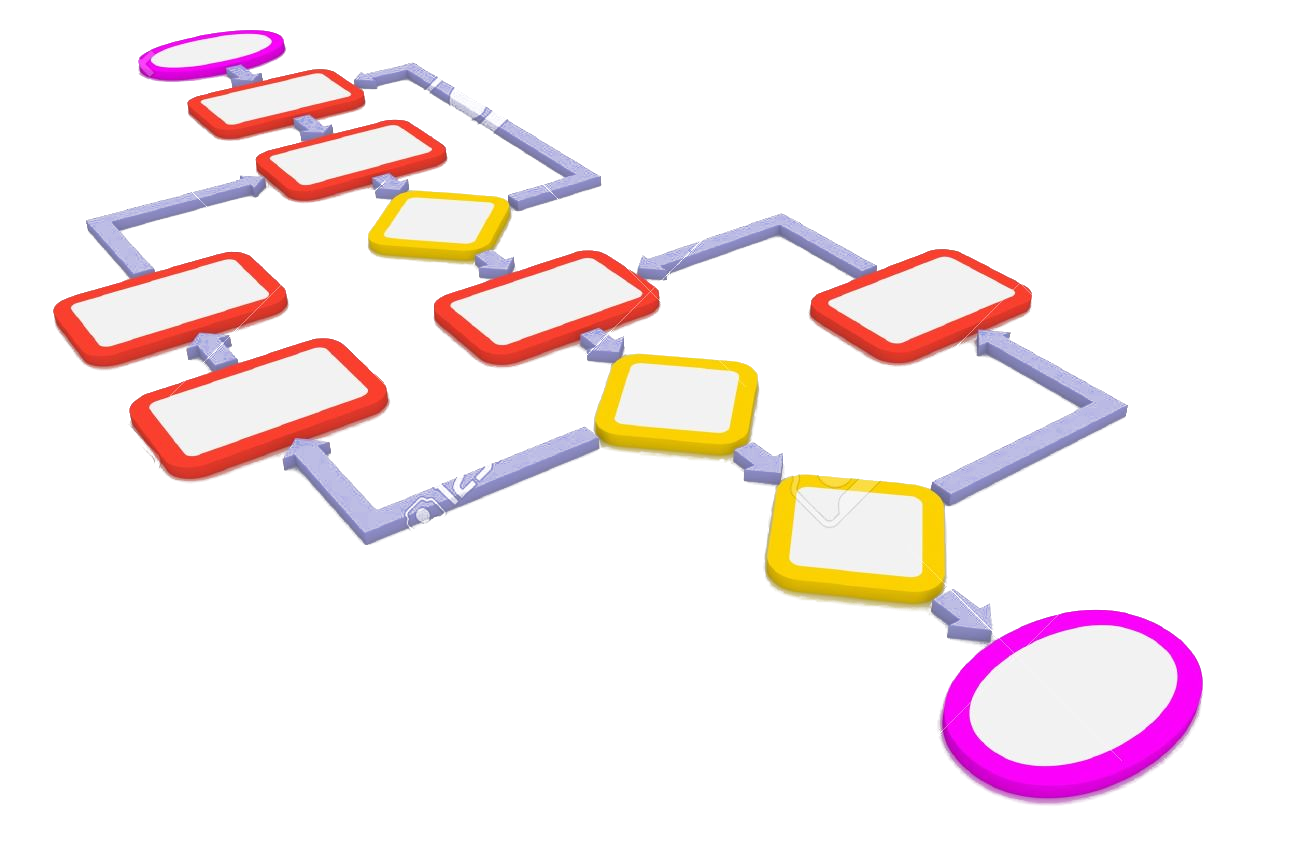
\includegraphics[width=116.85pt,height=118.05pt]{images/df3d.png}};
%Straight Lines [id:da6503370264075067] 
\draw    (379.4,141.8) -- (443.4,141.8) ;
\draw [shift={(446.4,141.8)}, rotate = 180] [fill={rgb, 255:red, 0; green, 0; blue, 0 }  ][line width=0.08]  [draw opacity=0] (8.93,-4.29) -- (0,0) -- (8.93,4.29) -- cycle    ;
\draw [shift={(376.4,141.8)}, rotate = 0] [fill={rgb, 255:red, 0; green, 0; blue, 0 }  ][line width=0.08]  [draw opacity=0] (8.93,-4.29) -- (0,0) -- (8.93,4.29) -- cycle    ;

% Text Node
\draw (245.6,218) node [anchor=north west][inner sep=0.75pt]   [align=left] {Estructuras de Datos};
% Text Node
\draw (49.6,206.4) node [anchor=north west][inner sep=0.75pt]   [align=left] {\begin{minipage}[lt]{59.43200000000001pt}\setlength\topsep{0pt}
\begin{center}
Algoritmos\\(Programas)
\end{center}

\end{minipage}};
% Text Node
\draw (528,214) node [anchor=north west][inner sep=0.75pt]   [align=left] {Datos};


\end{tikzpicture}
